\subsection{Plant-Controller Structure}
\subsubsection{Hierarchical Controller Structure}

The design started by considering what controller we need to run the plant globally. 
Some components are nonlinear in their behaviour (however non linearity is not implemented in the model), there are constraints on the operation of some components, and it would be beneficial to use predicted disturbances to control grid frequency in an optimal manner.
An LQR based controller does not give the power to play with these properties, so a \emph{Model Predictive Controller} (MPC) is preferred, but complicated to implement.

A MPC will allow us to  generate an optimal control scheme for our plant - but are limited in that they run on discrete time, and will not offer a instantaneous response.

\newpage

In the ideal scenario, the controller structure to be as follows:

\begin{figure}[thb]
        \centering
\usetikzlibrary{arrows}
        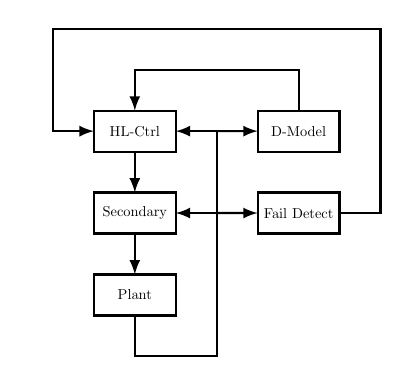
\begin{tikzpicture}[thick,scale=0.52, every node/.style={scale=0.52}]
\node (h) at (0,3) {HL-Ctrl};
\draw  (1,2.5) rectangle (-1,3.5);
\node (b) at (0,1) {Secondary};
\node  (t) at (0,-1) {Plant};
\draw  (1,0.5) rectangle (-1,1.5);
\draw  (1,-1.5) rectangle (-1,-0.5);
\draw (-2.5,-2);
\node at (4,3) {D-Model};
\node at (4,1) {Fail Detect};
\draw  (3,3.5) rectangle (5,2.5);
\draw  (3,1.5) rectangle (5,0.5);
\draw [-latex](0,2.5) -- (0,1.5);
\draw [-latex](0,0.5) -- (0,-0.5);
\draw [-latex](0,-1.5) -- (0,-2.5) -- (2,-2.5) -- (2,3) coordinate (v2) {} -- (1,3);
\draw [-latex](2,1) coordinate (v1) {} -- (1,1);
\draw [-latex](v1) -- (3,1);
\draw [-latex](v2) -- (3,3);
\draw [-latex](4,3.5) -- (4,4.5) -- (0,4.5) -- (0,3.5);
\draw [-latex](5,1) -- (6,1) -- (6,5.5) -- (-2,5.5) -- (-2,3) -- (-1,3);
\node at (-2.5,2) {};
\end{tikzpicture}
        \caption{A simplified view of how the controllers and sensing tie together} \label{fig:schematic}
\end{figure}

\begin{description}
        \item[The High-Level Controller] (HL-Ctrl) would dictate how each component (Electrolyser, SOFC and Gas Turbine) would be used, given information on failure states, predicted future demand, and the current system state. This is explored in Sections \ref{sec:power-pid} and \ref{sec:lqr}.
        \item[The Secondary Controller] would be a Virtual Inertia, a method used to simulate a large grid inertia with more inexpensive methods. {This is explored in Section \ref{sec:vi}, \emph{but not in depth.}}
        \item[Failure detection] can be achieved via a Kalman filter as suggested by \cite{power:kalman}, and the information gained can inform the controller of possible constraints. {This is mentioned in Section \ref{sec:failurestate}.}
        \item[A Disturbance Model] can aid in the case of MPC, future disturbance is \emph{not known} in a causal system. By having a disturbance model, the system can predict (using a Markov Chain \cite{power:markovP}) what the future state will be.
        \item[The `Plant' block] is where most of the design effort was focused, forming a model of the power-production and material balance will help greatly in deciding if this is a viable method of energy storage. {This is explored below in moderate depth, using information from Section \ref{sec:sysdyn} to be implemented in Section \ref{sec:plant}.}
\end{description}

This topology would be ideal as the High-Level controller would dictate the control of the plant for the most cost-effective response.
The Secondary (Virtual Inertia) controller would manage very fast changes in the system state - to ensure a low enough bandwidth for any high-level controller operation.
The High-Level controller would require state information from the disturbance model on future demand predictions, as well as the actual plant state (component actuation, grid frequency).
Failure detection would be important in later iterations to ensure the plant will run safely in all possible conditions - to ensure a stable electricity supply for consumers.

\subsubsection{Process of Implementation}

Implementation began by designing the core components of the plant.
Approximate models for each component were formed.
This allowed observations of responses to step requests, and from there constructed simple methods of control.
Proportional, PID and LQR schemes were explored to check stability and find the optimal result.
LQR was implemented, and model complexity was added.

Alongside development of the plant and classical controllers, methods on disturbance modelling were explored and data were collected to aid with the exploration piece of Model Predictive Control.
